\section{Torque Sensor}
The purpose of the Torque Sensor is to measure the mechanical power which is given to the sensor in the form of rotational energy from the Roll. The sensor must be able to measure both torque $\tau$ and angular velocity $\omega$ as the power P is given by:
\begin{equation}
	P=\omega\cdot\tau
\end{equation}

As the Torque Sensor was chosen by the customer and as it is pre-mounted on the Roll Stand, the block will not be designed but will be analysed instead.

\subsection{Implementation}
The torque sensor picked by the customer is a DR-2212 Contactless Torque Sensor from Lorenz Messtechnik GmbH. The sensor is able to measure both the angular velocity and the torque applied to the input-shaft. 
It is specified to be able to measure torque levels ranging from $-5 Nm$ to $+5 Nm$ (negative torque refers to the fact that the sensor can measure irregardles of the shaft's spin-direction).

\begin{figure}[H]
	\centering
	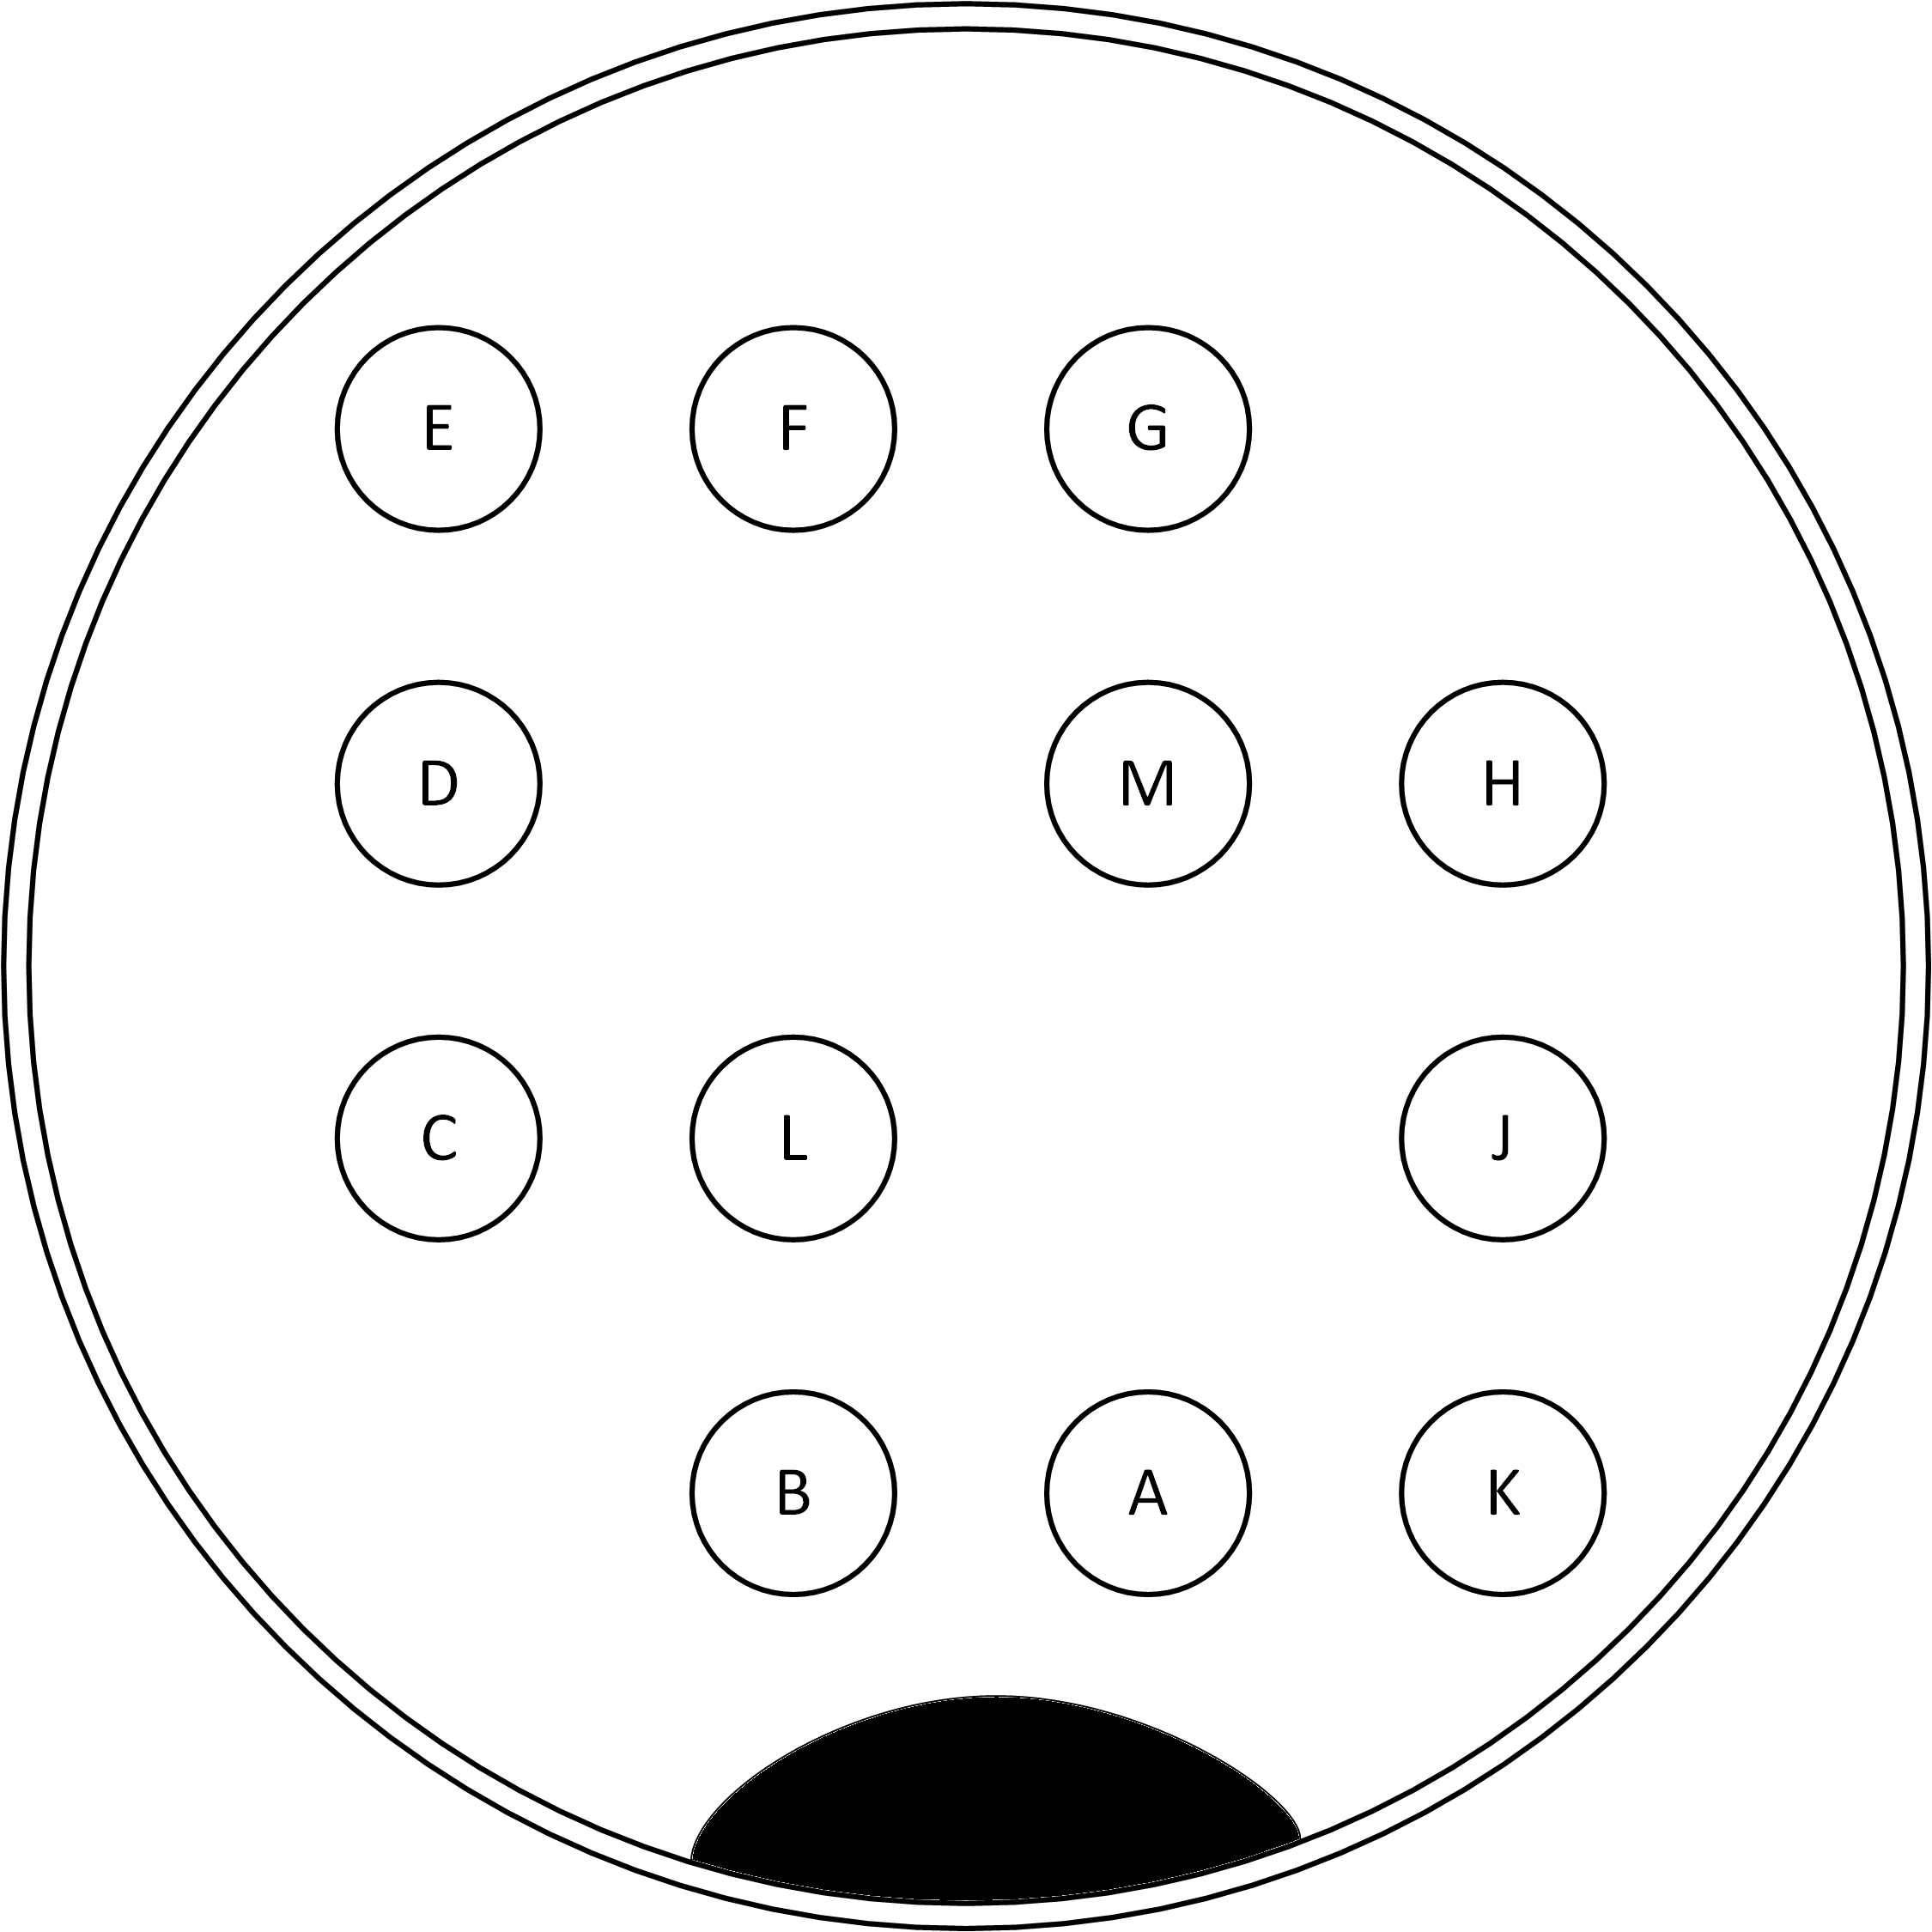
\includegraphics[width=0.3\linewidth]{Hardware/Pictures/Torque_Sensor_Pins}
	\caption{Torque Sensor Pins}
	\label{fig:Torque_pins}
\end{figure}

\subsection{Analysis}
Text

\subsection{Unity test}
Text